\documentclass[reprint,amsmath,amssymb,aps,]{revtex4-2}
\usepackage{graphicx}
\usepackage{dcolumn}
\usepackage{bm}
\usepackage{scrextend}
\usepackage{vmargin}
\usepackage{multirow}
\usepackage[utf8]{inputenc}
\usepackage[spanish, es-tabla]{babel}
\usepackage{enumerate}
\usepackage{float}
\usepackage{lipsum}
\usepackage{caption}
\usepackage{subcaption}
\usepackage{amsmath, amsthm, amssymb, amsfonts}
\usepackage[usenames]{color}
\usepackage[breaklinks=true,hidelinks]{hyperref}
\pagestyle{empty}
\begin{document}
\preprint{APS/123-QED}
\begin{abstract}
Se propuso un sistema de dos dimensiones conformado por átomos de carbono bajo el potencial de Lennard-Jones donde estuvo en contacto
a un termostato isocinético, se realizaron varias simulaciones variando su densidad y la temperatura del termostato, todos bajo la misma
temperatura inicial. Se obtuvo que los átomos tienden a estar más agrupados cuando la densidad y la temperatura del termostato estan con niveles bajo, en
comparación cuando se tiene al sistema con una densidad y temperatura del termostato alta, en donde los átomos tienden a agruparse a diferentes distancias.\\
\textbf{Palabras clave:} Potencial de Lennard-Jones, distribución radial, dos dimensiones, termostato isocinético.
\end{abstract}
\begin{titlepage}
\begin{center}

\includegraphics[scale=0.40]{../../../Logos/uanl.png} 
\hspace{2.5cm}

\includegraphics[scale=0.40]{../../../Logos/fcfm.png}
\end{center}
\vspace{2cm}
\begin{center}
\textbf{
UNIVERSIDAD AUTÓNOMA DE NUEVO LEÓN\\
FACULTAD DE CIENCIAS
FÍSICO MATEMÁTICAS}\\
\vspace*{2cm}
\begin{large}
\vspace{1cm}
\textbf{Simuladores Moleculares\vspace{0.5cm}\\
Dinámica molecular con el potencial \\ de Lennard-Jones en dos dimensiones\\ para diferntes densidades usando un termostato isocinético}\\
Omar Gonzalez Amezcua\\
\end{large}
\vspace{3.5cm}
\begin{minipage}{0.6\linewidth}
\vspace{0.5cm}
\changefontsizes{14pt}
Nombre:\\
Giovanni Gamaliel López Padilla\\
\end{minipage}
\begin{minipage}{0.2\linewidth}
\changefontsizes{14pt}
Matricula:\\
1837522
\end{minipage}
\end{center}
\vspace{4cm}
\begin{flushright}
\today
\end{flushright}
\pagebreak
\end{titlepage}
\maketitle
\section{Introducción}
La simulación de estructuras bajo ciertas condiciones es de gran ayuda cuando se necesita conocer que puede llegar a pasar en la experimentación,
es por ellos que es necesario la implementación de artefactos físicos para conocer la interacción entre este objeto y el sistema propuesto.
El termostato isocinético ayuda al sistema a que encuentre un estado de equilibrio constante, esto variando la temperatura a la cual se encuentra el termostato,
la representación física de este objeto puede interpretarse como la temperatura del sistema exterior (ambiente) en el cual se encuentra inmerso nuestro sistema de estudio.
\section{Objetivo general}
Realizar la implementación del termostato isocinético en la simulación bidimensional de átomos de
 Carbono afectados por el potencial de Lennard-Jones.
 \section{Objetivo específico}
 \begin{itemize}
     \item Observar el cambio en las distancias radiales variando la densidad y la temperatura del termostato.
     \item Monitorear la energía total del sistema a lo largo de la simulación.
     \item Monitorear la temperatura del sistema a lo largo de la simulación para verificar que el termostato se encuentra realizando
     su acción.
 \end{itemize}
\section{Marco teórico}
El potencial de Lennard-Jones describe la energía potencial de interacción entre dos átomos o moleculas netros sujetos a dos fuerzas distintas, una fuerza que tiene mayor acción cuando la distancia entre las dos sistemas es grande y la otra fuerza de interacción tiene una mayor acción a corta distancia. Este potencial tiene la siguiente forma:
\begin{equation}
    \label{Potencial de Lennard-Jones}
    V(r) = 4 \epsilon \left[\left(\frac{\sigma}{r} \right)^{12} - \left(\frac{\sigma}{r} \right)^6 \right]
\end{equation}
donde:
\begin{itemize}
    \item $V$ es el potencial intermolecular entre dos átomos o partículas.
    \item $\epsilon$ es la profundidad del valle que define que tan fuerte es la atracción entre partículas.
    \item $\sigma$ es la distancia a la cual el potencial entre dos partículas es igual a cero.
    \item $r$ es la distancia de separación entre dos partículas
\end{itemize}
Los parámetros $\epsilon$ y $\sigma$ son ajustados para reproducir datos experimentales o pueden ser dedudidos de resultados a partir de cálculos de química cuántica. La fígura \ref{Potencial de Lennard-Jones} es el potencial de Lennard-Jones con $\epsilon=1$ y $\sigma=1$.\\
En donde expone una gráfica de potenciales universales para estructuras de gráfito, y la que tenemos se asemeja en comportamiento a pesar de no tener la estrucura de un grafito.
Teniendo el potencial de la ecuación \ref{Potencial de Lennard-Jones}, podemos deducir la fuerza, ya que esta puede ser deducida a partir de aplicar el gradiente a la función $V(r)$, teniendo así la siguiente expresión:
\begin{equation}
    \label{eq:fuerzateo}
    \vec{F}(r)= 48\epsilon \left(\frac{\sigma^{12}}{r^{13}}- \frac{1}{2}\frac{\sigma^6}{r^7} \right) \hat{r}
\end{equation}
reescribiendo las ecuaciones \ref{Potencial de Lennard-Jones} y \ref{eq:fuerzateo} para tener la suma de estas en un sistema de n particulas se tiene lo siguiente:
\begin{equation}
    \label{eq:pot-n}
    U_t=\left\langle\sum_{i=1}^N \sum_{j<i}^N V_i,j(|r_j-r_i|)\right\rangle_t
\end{equation}
\begin{equation}
    \changefontsizes{9pt}
    \label{eq:f-n}
    F_i = \frac{48}{\sigma^2} \sum_{j \ne i} \left[\left(\frac{\sigma}{r_{ij}}\right)^{14}-\frac{1}{2}\left(\frac{\sigma}{r_{ij}} \right)^8  \right] (r_j-r_i)
\end{equation}
\begin{figure}[H]
    \centering
    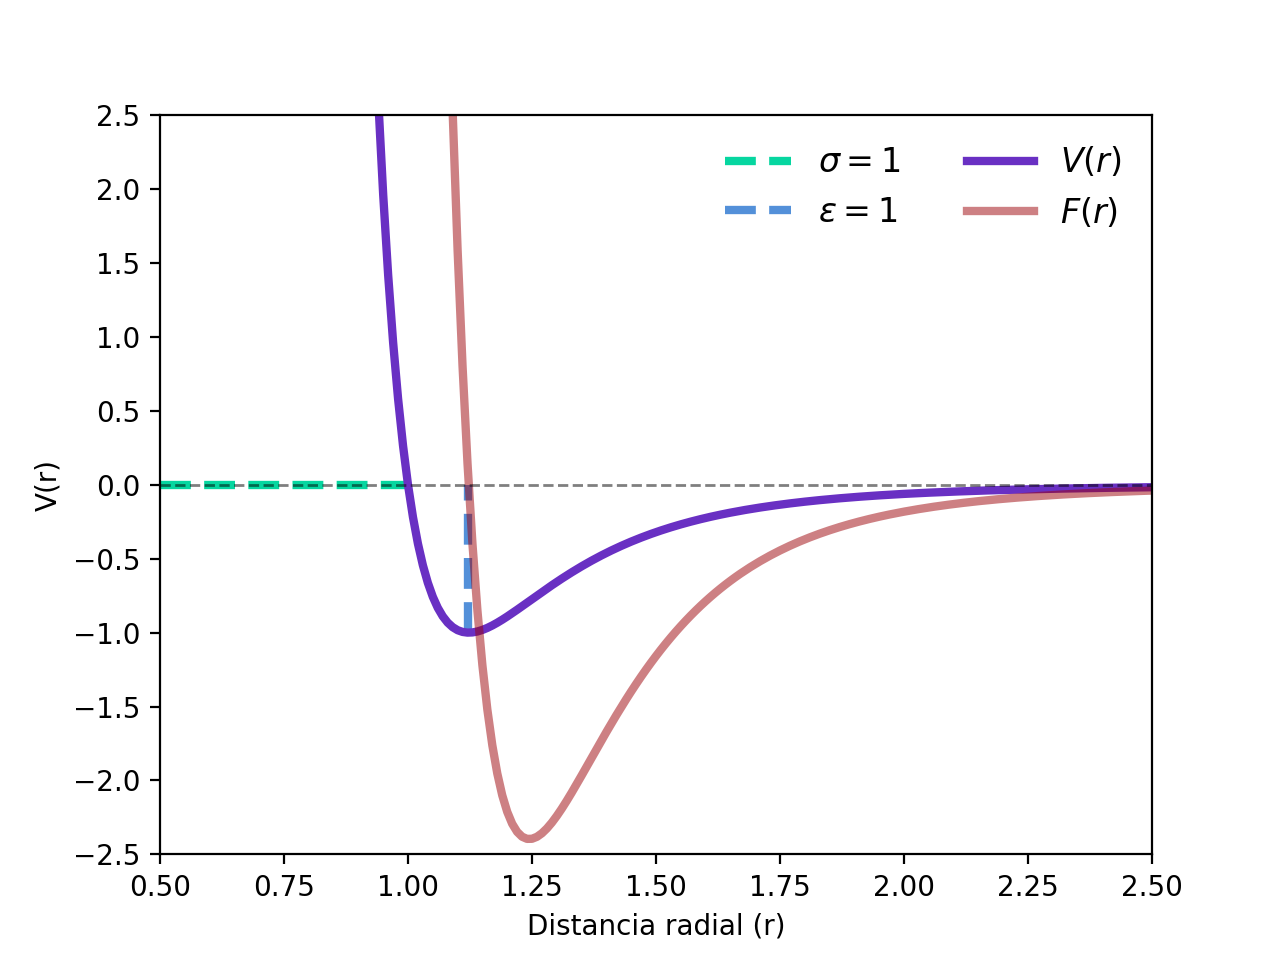
\includegraphics[scale=0.45]{../Graphics/Potencial.png}
    \caption{Potencial y fuerza de Lennard-Jones}
    \label{fig:pot-len-jones}
\end{figure}
\begin{table*}
    \centering
    \begin{tabular}{ccp{1cm}p{0.5cm}cccc}
        \hline
        Dimensión & Número de átomos & $\epsilon$ & $\sigma $ & $\rho $ & Número de pasos & T\textsubscript{0} & T\textsubscript{IT}\\ \hline
        \multirow{2}{*}{2} &\multirow{2}{*}{784} &\multirow{2}{*}{1} &\multirow{2}{*}{1}  &\multirow{2}{*}{Variable$^{*}$}  &\multirow{2}{*}{$2x10^{3}$} & \multirow{2}{*}{0.6} & \multirow{2}{*}{Variable}\\
         & & & & & & \\ \hline
    \end{tabular}
    \caption{Parámetros para las diferentes simulaciones, los valores tomados para las densidades fueron: 0.3, 0.6, 0.8; y
     para la temperatura del termostato isocinético (T\textsubscript{IT}) fueron 0.3, 0.5, 0.7, 0.9 y 1.1.}
    \label{table:parametros}
\end{table*}
Teniendo ya la dinámica se este sistema podemos ir monitoreando la energía cinética de la siguiente manera:
\begin{equation}
    \label{eq:kin-n}
    T_t=\left\langle \sum_{i=1}^N \frac{1}{2}m|v_i(t)|^2\right\rangle
\end{equation}
por lo tanto, la energía total para un tiempo t será:
\begin{equation}
    \label{eq:e-tot}
    E_t=T_t+U_t
\end{equation}
El control de temperatura isocinético es un método el cual las velocidades son escalonadas por un parámetros $\lambda$ a intervalos regulares,
el objetivo de esto es obtener una simulación estable con energía cinética media adecuada a la establecida con el termostato.\\
Este parámetro $\lambda$ es igual a lo siguiente:
\begin{equation}
    \lambda = \sqrt{\frac{T_0}{\tau}}
    \label{eq:lambda}
\end{equation}
donde $\tau$ esta definido como:
\begin{equation}
    \tau = \left\langle T \right\rangle
\end{equation}
Y la manera que actuará el termostato a lo largo de la simulación es el siguiente:
\begin{equation}
    {p}'_i(t+\Delta t) = \lambda p_i(t+\Delta t)
\end{equation}
en nuestro caso, como la masa de cada atómo es constante, la ecuación se reescribe como lo siguiente:
\begin{equation*}
    {v}'_i(t+ \Delta t) = \lambda v_i(t+\Delta t)
\end{equation*}
\section{Resultados}
Al termino de la simulación para diferentes densidades y temperaturas del termostato, este arroja diferentes resultados contenidos en archivos individuales.
La información que se obtiene es la energía cinética, la energía potencial y la temperatura del sistema a lo largo de la simualción y la distribución radial que 
hay entre cada átomo de carbono.\\
La simulación de la pĺaca bidimensional fue realizada siguiendo los parámetros mostrados en la tabla \ref{table:parametros}, en la cual la temperatura inicial siempre tuvo el mismo valor,
las densidades que se realizaron fueron de 0.3,0.6 y 0.8, en cambio las temperaturas del termostato isocinético se tomaron los siguientes valores: 0.3, 0.5, 0.7, 0.9 y 1.1.\\
Observando el comportamiento de la energía total a lo largo de la simualción se puede observar que sigue un comportamiento oscilatorio
independientemente de la densidad y la temperatura del termostato isocinético, esto nos da un indicio que el sistema llego a un punto de
equilibrio como se puede mostrar en la figura \ref{fig:energy}.
\begin{figure}[H]
\hspace{-0.75cm}
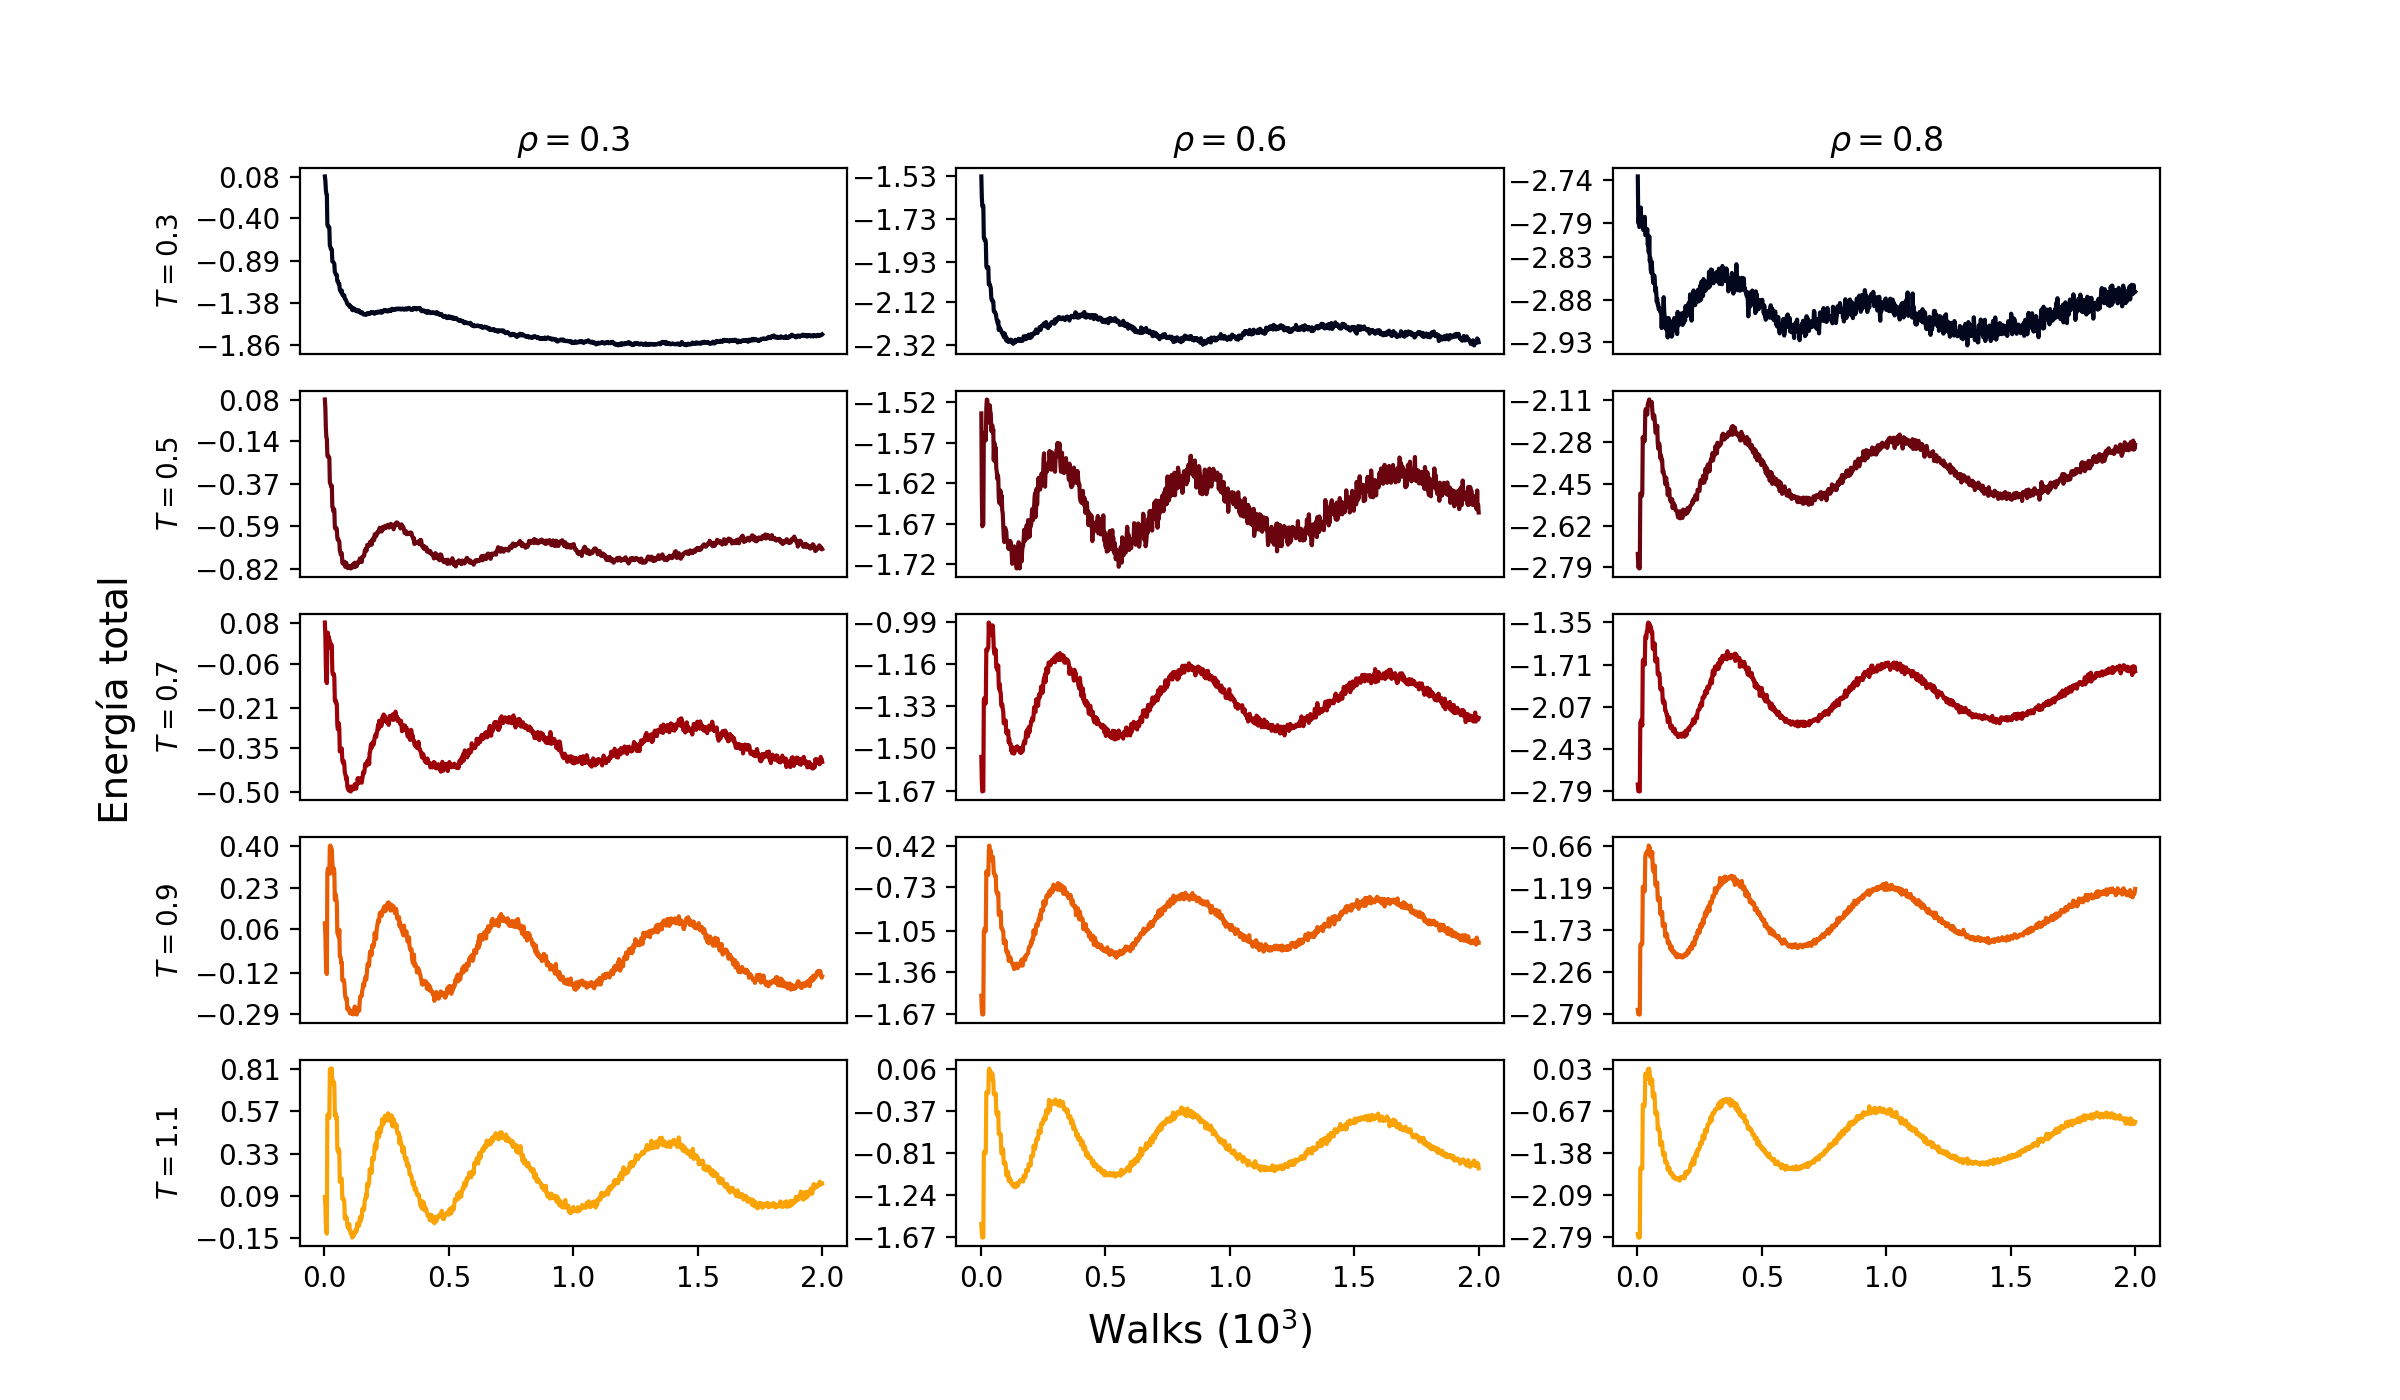
\includegraphics[scale=0.275]{../Graphics/Energy.png}
\caption{Energía total a lo largo de la simulación de las densidades seleccionadas variando la temperatura del termostato.}
\label{fig:energy}
\end{figure}
\begin{figure*}
    \hspace*{-1cm}
    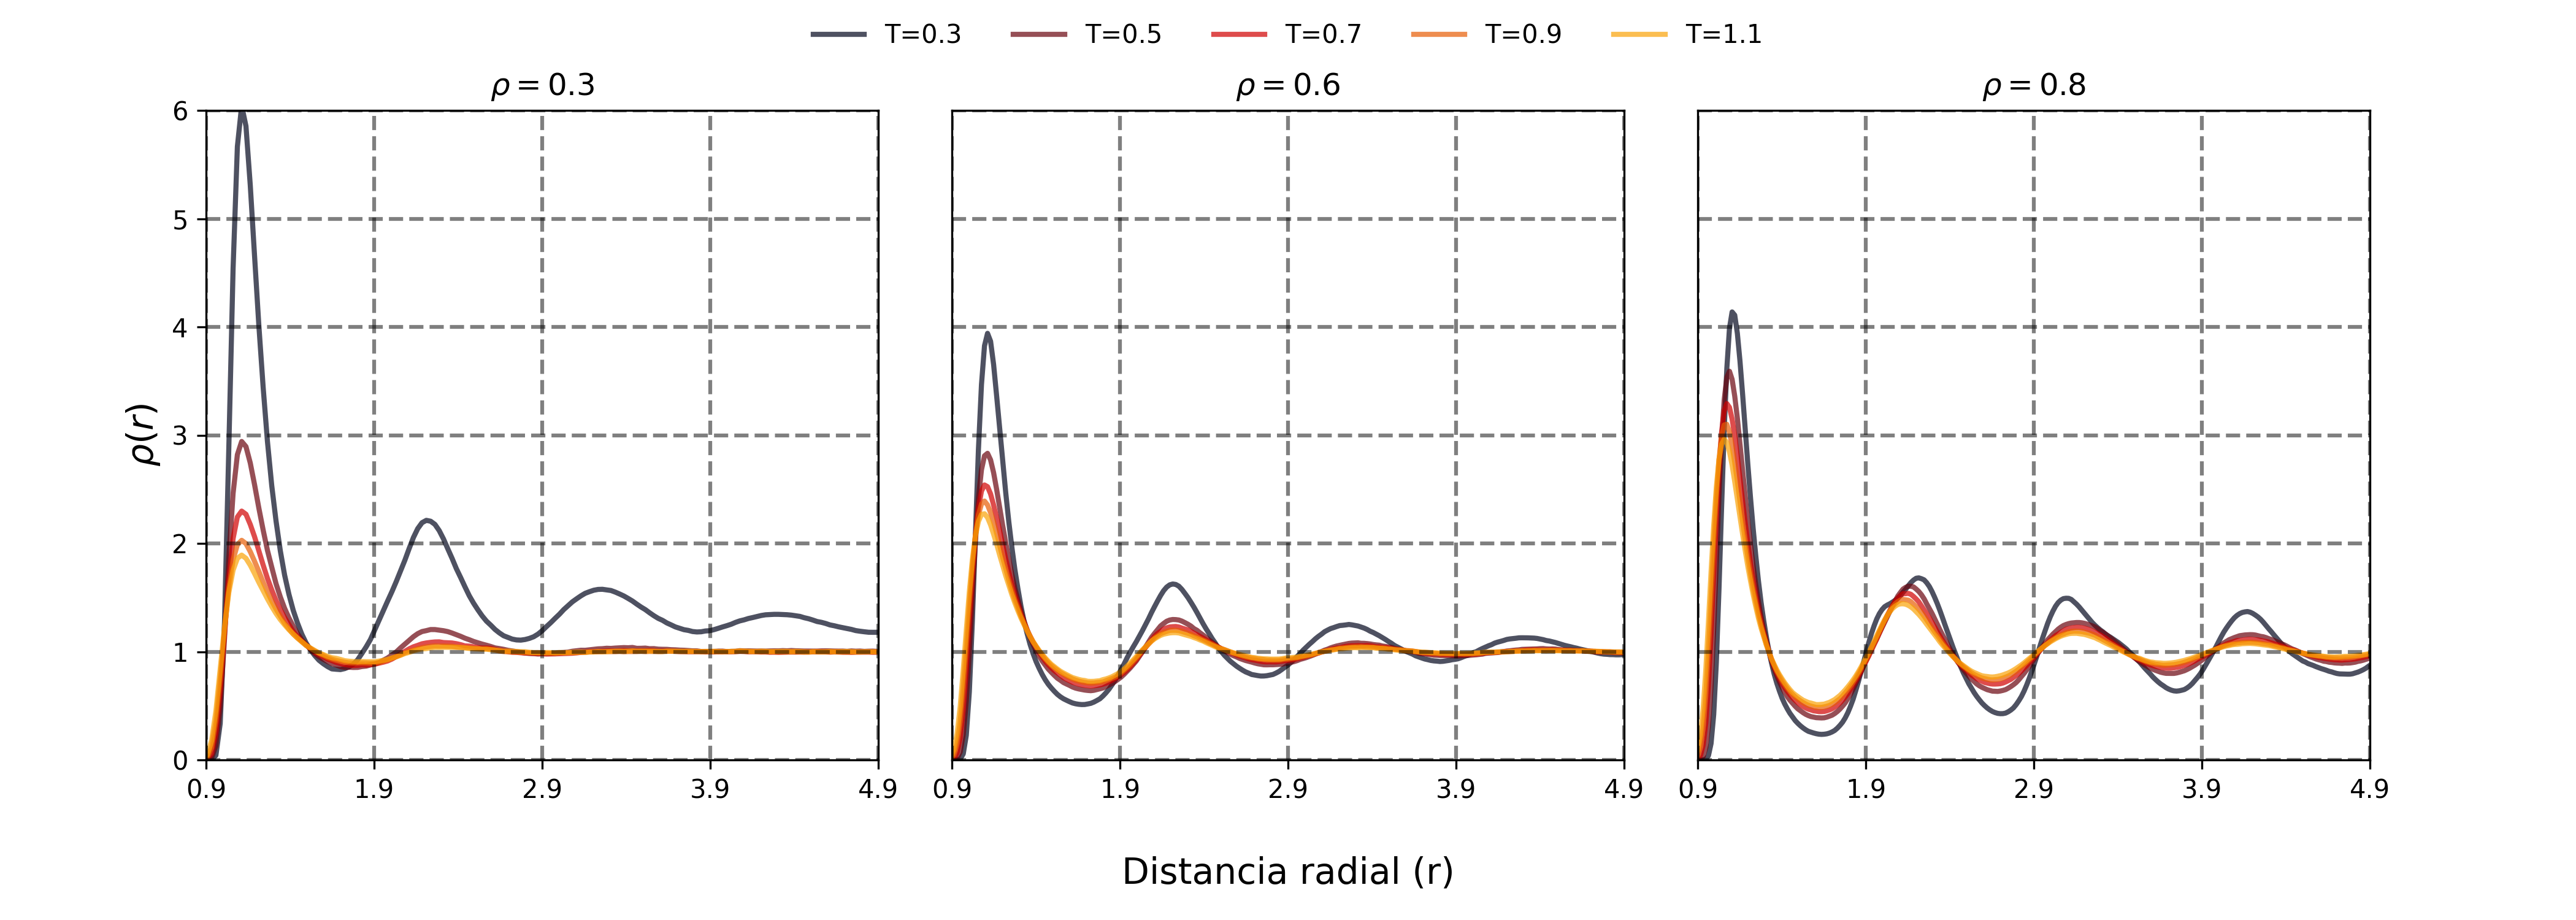
\includegraphics[scale=0.45]{../Graphics/Dis_rad.png}
    \caption{Distribución radial de la estructura}
    \label{fig:disradial}
\end{figure*}
Analizando las distancias radiales muestran que a una menor temperatura independientemente de la densidad, los átomos se agrupan más a la distancia de 1, en cambio
al aumentar la densidad, los átomos tienden a agruparse en diferntes distancias.
Realizndo una comparación con la simulación sin el termostato, sucede de igual manera que mientras mayor sea la densidad
la concentración de átomos se distribuye en diferentes zonas. Todo lo anterior se puede observar en la figura \ref{fig:disradial}.\\\\

Analizando la temperatura de los diferentes sistemas se observa que todos llegan a estar en un equilibrio con el termostato, independientemente
de la densidad del sistema, el tiempo que tarda en llegar a este equilibrio depende mayormente de la temperatura del termostato, todo esto se puede observar
en la figura \ref{fig:temp}.
\begin{figure}[H]
    \hspace{-0.75cm}
    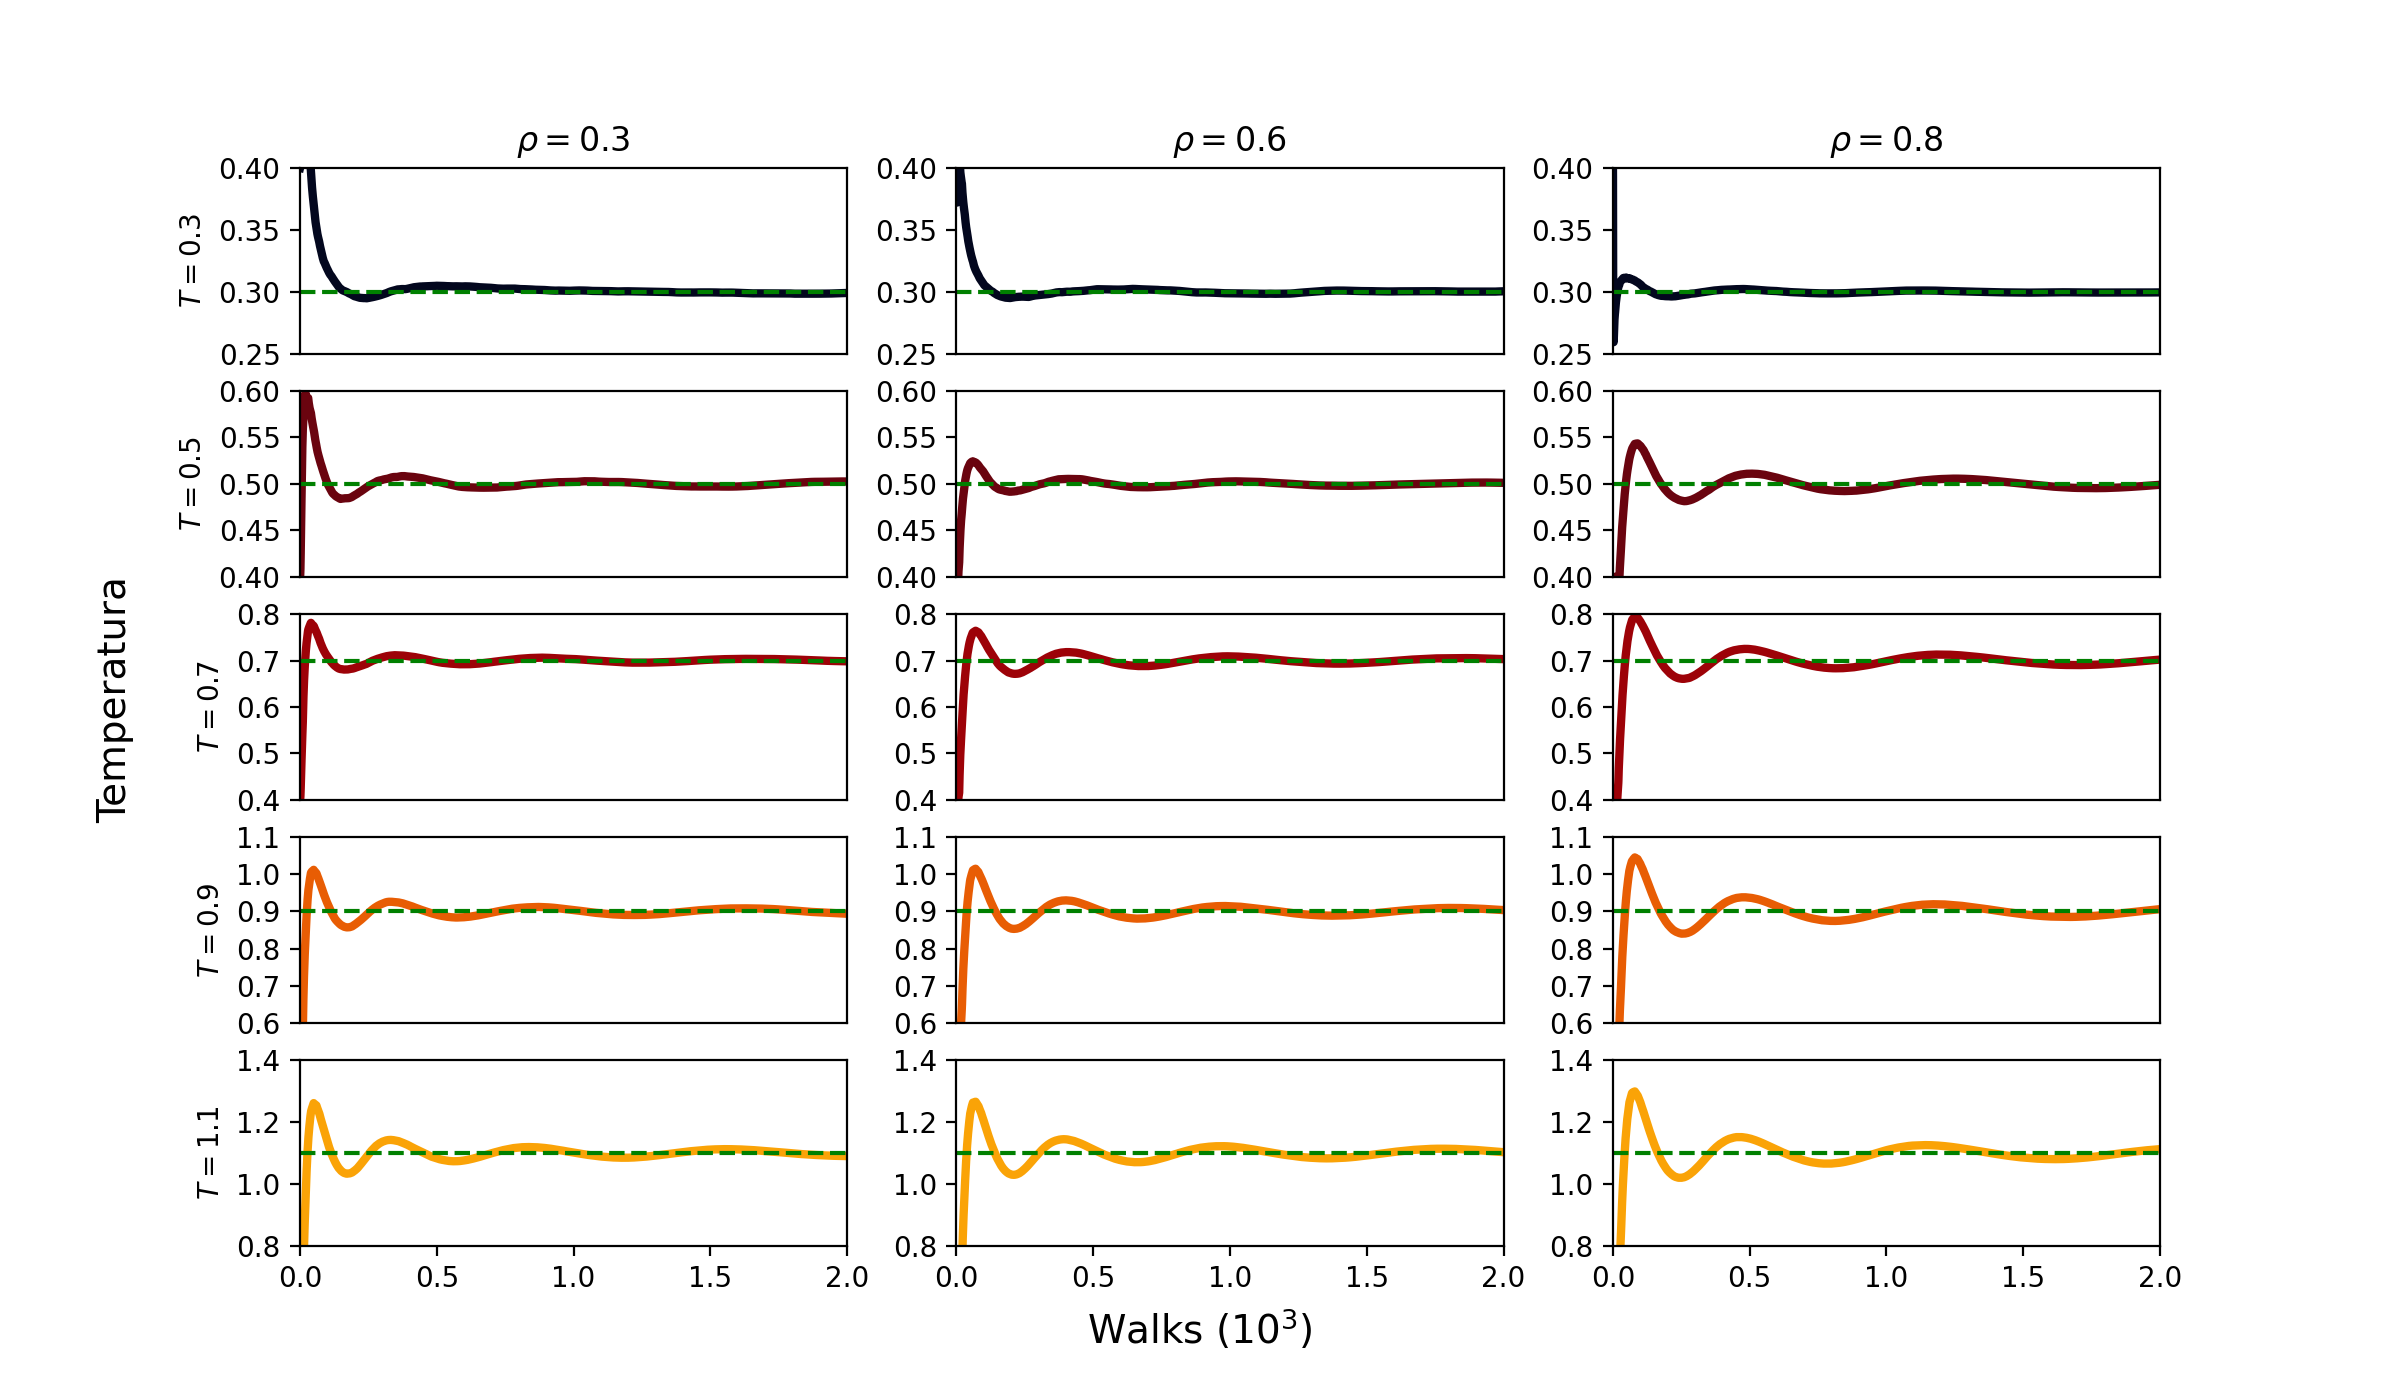
\includegraphics[scale=0.275]{../Graphics/Temp.png}
    \caption{temperatura del sistema para varias densidades y temperaturas del termostato a lo largo de la simulación}
    \label{fig:temp}
    \end{figure}
\section{Conclusiones}
La implementación del termostato isocinético realizo que el sistema estuviera en un estado de equilibrio, ya que, la misma simualción sin esta implementación
realizaba mayores variaciones en la energía, esto puede llegar ser util para la simulación de un sistema el cual se quiera llevar a este estado o aplicarlo experimentalmente
para un sistema el cual se necesite estar en equilibrio.
\section{Código}
\begin{itemize}
\item \href{https://github.com/giovannilopez9808/Notas_Agosto_2020/blob/master/Simulaciones/Proyecto_2/Scripts/MD-n2.f}{MD-n2.f}\\
Este código contiene la simulación de la placa bidimensional aplicando un potencial de Lennard-Jones y el termostato isocinético.
\item \href{https://github.com/giovannilopez9808/Notas_Agosto_2020/blob/master/Simulaciones/Proyecto_2/Scripts/Run.py}{Run.py}\\
Este código contiene la automatización de la simulación para las diferentes densidades y temperaturas del termostato.
\item \href{https://github.com/giovannilopez9808/Notas_Agosto_2020/blob/master/Simulaciones/Proyecto_2/Scripts/Potencial_Graphics.py}{Potencial\_Graphics.py}\\
Este código realiza la figura \ref{fig:pot-len-jones}
\item \href{https://github.com/giovannilopez9808/Notas_Agosto_2020/blob/master/Simulaciones/Proyecto_2/Scripts/Cor_Graphics.py}{Cor\_Graphics.py}\\
Este código realiza la gráfica \ref{fig:disradial}
\item \href{https://github.com/giovannilopez9808/Notas_Agosto_2020/blob/master/Simulaciones/Proyecto_2/Scripts/Temp_Graphics.py}{Temp\_Graphics.py}\\
Este código realiza la figura \ref{fig:temp}
\item \href{https://github.com/giovannilopez9808/Notas_Agosto_2020/blob/master/Simulaciones/Proyecto_2/Scripts/Energy_Graphics.py}{Energy\_Graphics.py}\\
Este código genera la figura \ref{fig:energy}
\end{itemize}
\bibliographystyle{plain}
\nocite{*}
\bibliography{Main}
\end{document}